\chapter{Höhere Ableitungen}

\setcounter{section}{9}
\setcounter{subsection}{0}
\setcounter{subsubsection}{1}
\setcounter{secnumdepth}{4}
\subsection{Mehrfaches Ableiten}
\href{https://youtu.be/CA2VJcrvSVo}{Video 01}\\
Sei $ f:\mathbb{R}\supset\mathbb{I}\longmapsto\mathbb{R} $ auf $ \mathbb{I} $ diffbar, dann ist $ f':\mathbb{I}\longmapsto\mathbb{R} $ mit $ x\longmapsto f'(x) $ eine Funktion.\\
Ist $ f' $ auf $ \mathbb{I} $ diffbar, dann heißt\\
\begin{align*}
f'':=(f')'\\
\end{align*}
die zweite Ableitung von $ f $.\vspace*{4mm}\\
Beispiel:\\
\begin{align*}
f(x)&=x^2\\
f'(x)&=2x\\
f''(x)&=(f'(x))'=(2x)'=2\\
\end{align*}
Für $ k\in \mathbb{N} $ definieren wir die $ k- $te Ableitung:\\
\begin{align*}
f^{(k)}:=(f^{k-1})'\;\;\text{, wobei } f^{(0)}:=f\;\;\text{ist. }\\
\end{align*}
Beispiel:\\
\begin{align*}
f(x)&=x^3\\
f'(x)&=3x\\
f''(x)&=3\\
f^{(3)}(x)&=0\\
f^{(123)}(x)&=0\\
\end{align*}
Hier gibt es unendlich viele Ableitungen.\\
\newpage
\noindent
Bemerkung:\\
Beispiel:\\
\textbullet \;\;$ f(x)=|x| $ \\
\begin{quote}
	$ f(x)=|x| $ ist in $ x_0=0 $ nicht ableitbar, weil in $ x_0 $ nicht diffbar!\\
\end{quote}
\textbullet \;\;$ g(x) =     \left\{ \begin{array}{rcl}
\frac{1}{2 }x^2 & \mbox{für} & x\geq0\\
-\frac{1}{2}x^2 & \mbox{für} & x< 0 \\

\end{array}\right.$ \\
\begin{quote}
Überprüfung der Differenzierbarkeit in $ x_0=0 $.\\
Grenzwertbetrachtung:\\
\begin{align*}
\lim\limits_ {\substack{x \to x_0 \\ x<0}}\frac{g(x)-g(x_0)}{x-x_0}=\lim\limits_ {x\to x_0}\frac{-\frac{1}{2}x^2}{x}=\lim\limits_ {n\to x_0}-\frac{1}{2}x=0=\lim\limits_ {x\to x_0}\frac{1}{2}x=\lim\limits_ {x\to x_0}\frac{\frac{1}{2}x^2}{x}=\lim\limits_ {\substack{x \to x_0 \\ x> 0}}\frac{g(x)-g(x_0)}{x-x_0}
\end{align*}
Der links- und rechtsseitige Grenzwert ist gleich und deshalb ist die Funktion
$ g(x) $ in $ x_0=0 $ differenzierbar. Bei $ x_0\neq 0 $ ist $ g(x) $ als Komposition einer differenzierbaren Funktion differenzierbar.\\

\begin{align*}
&g'(x) =     \left\{ \begin{array}{rcl}
(\frac{1}{2}x^2)' & \mbox{für} & x\geq 0\\
(-\frac{1}{2}x^2)' & \mbox{für} & x<0 \\
\end{array}\right.\\
&g'(x) =     \left\{ \begin{array}{rcl}
x & \mbox{für} & x\geq 0\\
-x & \mbox{für} & x<0 \\
\end{array}\right.=|x|\\
\end{align*}
$ g'(x)=|x| $ ist nicht diffbar.\\
Fazit:\\
$ g(x) $ ist nur einmal differenzierbar.\\
\end{quote}
\subsubsection{Mehrfaches Ableiten - Aufgabe}
\href{https://youtu.be/1SbIqyzxLeg}{Video 02}\\
Sei $ f(x)=x^2+2x+7 $.\\
Berechne:\\
\begin{align*}
g(x)=f(1)+f'(1)(x-1)+\frac{f''(x)}{2}(x-2)^2
\end{align*}
und vergleiche $ g(x) $ mit $ f(x) $.\\
\begin{align*}
f(x)&=x^2+2x+7\\
f(1)&=1^2+2+7=10\\
f'(x)&=2x+2\\
f'(1)&=2+2=4\\
f''(x)&=2\\
f''(2)&=2\\
g(x)&=10+4(x-1)+(x-1)^2\\
g(x)&=10+4x-4+x^2-2x+1=x^2+2x+7=f(x)\\
\end{align*}
Die Frage ist nun: Gilt dies für alle Polynome?\\
\subsection{ Herleitung des Taylorpolynoms}
\href{https://youtu.be/EFkwp2qckNU}{Video 03}\\
Sei $ x_0\in\mathbb{R} $ und betrachte $ f(x)=a_0+a_1(x-x_0)+\ldots+a_k(x-x_0)^k\ldots+a_n(x-x_0)^n $.\vspace*{4mm}\\
Untersuchung von $ h(x)=a_k(x-x_0)^k $\\
\begin{align*}
h(x)&=a_k(x-x_0)^k\\
h'(x)&=a_k\cdot k(x-x_0)^{k-1}\\
h''(x)&=a_k\cdot k\cdot (k-1)(x-x_0)^{k-2}\\
&\;\;\cdot\\
&\;\;\cdot\\
&\;\;\cdot\\
h^{(k)}(x)&=a_k\cdot \underbrace {k(k-1)\ldots 3\cdot 2 \cdot 1}_{=k!}(x-x_0)^0=a_k k!\\
h^{k+1}(x)&=0\\
\end{align*}
Durch einsetzen von $ x=x_0 $ in $ f(x) =a_0+a_1(x-x_0)+\ldots+a_k(x-x_0)^k\ldots+a_n(x-x_0)^n$ kann man die Koeffizienten $ a_k $ berechnen.\\
Dann gilt für $ x=x_0 $ eingesetzt in die Funktion $ f(x) $:\\
\begin{align*}
f(x_0)&=a_0+a_1(x-x_0)+\cdots +a_k(x-x_o)^k\\
f(x_0)&=a_0
\end{align*}
Alle anderen Summanten werden Null $ (x_0-x_0)=0 $.\vspace*{2mm}\\
Dann gilt für $ x=x_0 $ eingesetzt in die Funktion $ f'(x) $:\\
\begin{align*}
f'(x_0)&=a_1+\cdots+a_k\cdot k(x-x_0)^{k-1}\\
f'(x_0)&=a_1
\end{align*}
Dann gilt für: $ f^k(x_0) $
\begin{align*}
f^k (x_0)=a_k\cdot k!\Leftrightarrow a_k=\frac{f^k(x_0)}{k!}\\
\end{align*}
Dann ist:\\
\begin{align*}
a_0=\frac{f(x_0)}{0!}\\
a_1=\frac{f'(x_0)}{1!}\\
a_2=\frac{f''(x_0)}{2!}\\
a_n=\frac{f^n(x_0)}{n!}\\
\end{align*}
Daraus ergibt sich dann für f(x):\\
\begin{align*}
f(x)&=\frac{f(x_0)}{0!}+\frac{f'(x_0)(x-x_0)^1}{1!}+\frac{f''(x_0)(x-x_0)^2}{2!}+\ldots +\frac{f^n(x_0)-(x-x_0)^n}{n!}\\
&=\sum\limits_{k=0}^{n}\frac{f^k(x_0)}{k!}(x-x_0)^k\\
\end{align*}
Nun stellen sich die Fragen:\\
Was ist, wenn $ f $ kein Polynom ist ?\\
Welcher Zusammenhang besteht zwischen $ f $ und dem Polynom ?\\
\subsubsection{Das Taylorpolynom (Definition) }
\href{https://youtu.be/bSzpFWy4gTE}{Video 04}\\
Sei $ f: \mathbb{I}\longmapsto\mathbb{R} $ n-mal diffbar und $ x_0\in  \mathbb{I} $, dann heißt
\begin{align*}
T_{n,x_0}(x)=\sum\limits_{k=0}^{n}\frac{f^k(x_0)}{k!}(x-x_0)^k
\end{align*}
das n-te Taylorpolynom von $ f $ im Entwicklungspunkt $ x_0 $.\vspace*{2mm}\\
Beispiel: $ f(x)=\ln(x) $ mit $ x_0=1 $ und $ n=2 $\\
\begin{align*}
&f^{(0)}(1)=\ln(1)=0\\
&f^{(1)}(x)=(\ln(x))'=\frac{1}{x}\Rightarrow f^{(1)}(1)=1\\
&f^{(2)}(x)=\bigg(\frac{1}{x}\bigg)'=\frac{-1}{x^2}\Rightarrow f^{(2)}(1)=-1\\
\end{align*}
Daraus ergibt sich das Taylorpolynom:\\
\begin{align*}
T_{2,x_0}(x)&=\frac{f^{(0)}(x_0)}{0!}+\frac{f^{(1)}(x_0)}{1!}(x-x_0)+\frac{f^{(2)}(x_0)}{2!}(x-x_0)^2\\
T_{2,1}(x)&=0+1(x-1)+\frac{-1}{2}(x-1)^2\\
&=(x-1)-\frac{1}{2}(x-1)^2\\
\end{align*}
\subsubsection{Aufgabe 1 zum Taylorpolynom}
\href{https://youtu.be/YGIDHu8E8S4}{Video 05}\\
Berechne für $ f(x)=\sqrt{x} $ das Taylorpolynom 3. Grades im Entwicklungspunkt $ x_0=1 $.\\
\begin{align*}
T_{3,1}(x)=\sum\limits_{k=0}^{3}\frac{f^k(1)}{k!}(x-1)^k
\end{align*}
\newpage
\noindent
\textbullet \;\;Bestimmung der Ableitungen von  $ f'(x),f''(x)\;\text{ und}\; f^{(3)}(x)$.\\
\begin{quote}
\begin{align*}
f'(x)&=\frac{1}{2\sqrt{x}}\\
f''(x)&=\bigg(\frac{1}{2\sqrt{x}}\bigg)'=\frac{1}{2}\bigg(x^{-\frac{1}{2}}\bigg)'=\frac{1}{2}\bigg(-\frac{1}{2}\bigg)x^{-\frac{3}{2}}=-\frac{1}{4}\frac{1}{\sqrt{x^3}}\\
f^{(3)}(x)&=\bigg(-\frac{1}{4}\frac{1}{\sqrt{x^3}}\bigg)'=-\frac{1}{4}\bigg(x^{-\frac{3}{2}}\bigg)'=-\frac{1}{4}\bigg(-\frac{3}{2}\bigg)x^{-\frac{5}{2}}=\frac{3}{8}\frac{1}{\sqrt{x^5}}\\
\end{align*}
\end{quote}
\textbullet\;\; Bestimmung von $ f(x),\; f'(1),\; f''(1),\; f^{(3)}(1) $.\\
\begin{quote}
\begin{align*}
f(1)&=1\\
f'(1)&=\frac{1}{2\sqrt{1}}=\frac{1}{2}\\
f''(1)&=-\frac{1}{4}\frac{1}{\sqrt{1^3}}=-\frac{1}{4}\\
f^{(3)}(1)&=\frac{3}{8}\frac{1}{\sqrt{x^5}}=\frac{3}{8}\\
\end{align*}
\end{quote}
\textbullet\;\; Einsetzen in das Taylorpolynom.\\
\begin{quote}
\begin{align*}
T_{3,x_0}(x)&=\sum\limits_{k=0}^{3}\frac{f^k(x_0)}{k!}(x-x_0)^k=f(x_0)+\frac{f'(x_0)}{1!}(x-x_0)+\frac{f''(x_0)}{2!}(x-x_0)^2+\frac{f^{(3)}(x_0)}{3!}(x-x_0)^3\\
T_{3,1}(x)&=\sum\limits_{k=0}^{3}\frac{f^k(1)}{k!}(x-1)^k=f(x_0)+\frac{f'(1)}{1!}(x-1)+\frac{f''(1)}{2!}(x-1)^2+\frac{f^{(3)}(1)}{3!}(x-1)^3\\
\end{align*}
Einsetzen von $ f(x)=1,\; f'(1)=\frac{1}{2},\; f''(1)=-\frac{1}{4},\; f^{(3)}(1)=\frac{3}{8} $.
\begin{align*}
T_{3,1}(x)=1+\frac{1}{2}(x-1)-\frac{1}{8}(x-1)^2+\frac{3}{48}(x-1)^3\\
\end{align*}
\end{quote}
\subsubsection{Aufgabe 2 zum Taylorpolynom}
\href{https://youtu.be/uHJAzrQ-4-I}{Video 06}\\
Sei $ f $ die Lösung der Differentialgleichung $ f'(x)=2f(x)+\frac{3}{f(x)} $ mit $ f(0)=1 $.\\
Bestimme Taylorpolynom von 2. Grades in $ x_0=0 $.\vspace*{2mm}\\
\newpage
\noindent
\textbullet \;\;Bestimmung der Ableitungen von  $ f'(x),\;f''(x)$.\\
\begin{quote}
\begin{align*}
f'(x)&=2f(x)+\frac{3}{f(x)}\\
f''(x)&=\bigg(2f(x)+\frac{3}{f(x)}\bigg)'=2f'(x)+\bigg(\frac{3}{f(x)}\bigg)'\\
\end{align*}
NR.: $\bigg(\frac{3}{f(x)}\bigg)'  $\\
Es gilt:\\
\begin{align*}
\bigg(\frac{1}{x}\bigg)'&=\bigg(x^{-1}\bigg)'=-x^{-2}=-\frac{1}{x^2}\\
\bigg(\frac{1}{f(x)}\bigg)'&=\bigg((f(x))^{-1}\bigg)'=-f'(x)(f(x))^{-2}=-\frac{f'(x)}{(f(x))^2}\\
\end{align*}
\begin{align*}
&\bigg(\frac{3}{f(x)}\bigg)'=3\bigg(\frac{1}{f(x)}\bigg)'=3\big(f(x)^{-1}\big )'=-3f'(x)\big ( f(x)\big)^{-2}=-3\frac{f'(x)}{(f(x))^2}\\
&\text{mit Quotientenregel }\\
&\bigg(\frac{3}{f(x)}\bigg)'=\frac{0\cdot f(x)-3\cdot f'(x)}{(f(x))^2}=-3\frac{f'(x)}{(f(x))^2}\\
\end{align*}
\begin{align*}
\Rightarrow\\
f''(x)&=\bigg(2f(x)+\frac{3}{f(x)}\bigg)'=\bigg(2f(x)\bigg)'+\bigg(\frac{3}{f(x)}\bigg)'\\
&=2f'(x)-3\frac{f'(x)}{(f(x))^2}\\
&=f'(x)\bigg (2-\frac{3}{(f(x))^2}\bigg)
\end{align*}
\end{quote}
\textbullet\;\; Bestimmung von $ f(0),\; f'(0),\; f''(0) $.\\
\begin{quote}
\begin{align*}
f(0)&=1\\
f'(0)&=2f(0)+\frac{3}{f(0)}=2+3=5\\
f''(0)&=f'(0)\bigg (2-\frac{3}{(f(0))^2}\bigg)=5\bigg (2-\frac{3}{1}\bigg)=-5\\
\end{align*}
\end{quote}
\textbullet\;\; Einsetzen in das Taylorpolynom.\\
\begin{quote}
\begin{align*}
T_{2,0}&=\sum\limits_{k=0}^{2}\frac{f^k(0)}{k!}(x-0)^k=\frac{f(0)}{0!}(x-0)^0+\frac{f'(0)}{1!}(x-0)^1+\frac{f''(0)}{2!}(x-0)^2\\
&=1+5x-\frac{5}{2}x^2\\
\end{align*}
\end{quote}
\subsection{Geometrische Interpretation der Taylorapproximation Teil I+II}
\href{https://youtu.be/fznq-R-W_NQ}{Video 07}\\
Die Funktion $ f(x)=\mathrm{e}^x $ kann durch ein Taylorpolynom im Entwicklungspunkt $ x_0=0 $ dargestellt werden. Dabei gilt dann:\\
\begin{align*}
f(x)=\mathrm{e}^x\approx T_{n,x_0}\;\;\text{ für}\;\;x\;\;\text{in der Nähe von }\;\;x_0\\
\end{align*}
In der Nähe von $ x_0 $ sieht das Taylorpolynom $T_{n,x_0}  $ wie $ f(x)=\mathrm{e}^x $ aus.\\
Es gilt auch:\\
\begin{align*}
f(x)=\mathrm{e}^x=T_{n,x_0}+\text{Fehler }\\
\end{align*}
Es gilt für $ f(x)=\mathrm{e}^x $:\\
\begin{align*}
f(x)&=\mathrm{e}^x\\
f'(x)&=\mathrm{e}^x\\
f^{k}(x)&=\mathrm{e}^x\\
f^{k}(0)&=1\\
\end{align*}
Das Taylorpolynom für $ f(x)=\mathrm{e}^x $ im Entwicklungspunkt $ x_0=0 $ heißt dann:\\
\begin{align*}
T_{n,0}(x)=\sum\limits_{k=0}^{n}\frac{f^k(0)}{k!}(x-0)^k=\frac{f(0)}{0!}(x-0)^0+\frac{f'(0)}{1!}(x-0)^1+\frac{f''(0)}{2!}(x-0)^2+\frac{f^{3}(0)}{3!}(x-0)^3+\ldots
\end{align*}
\underline{Für $ n=1 $ gilt:}\\
\begin{align*}
T_{1,0}(x)0&=f(0)+\frac{f'(0)}{1!}(x-0)\\
&=1+x\\
\end{align*}
\begin{center}
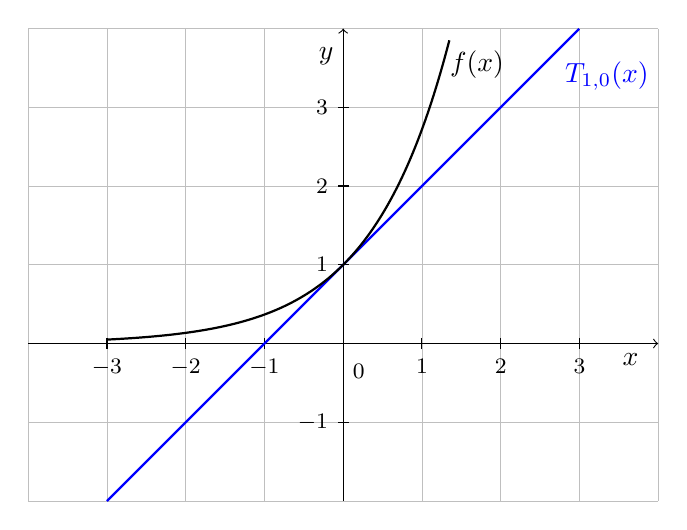
\begin{tikzpicture}


% Gitternetzlinien
\draw[xstep=1cm, ystep=1cm, very thin, color=lightgray] (-4,4) grid (4,-2);
% x-Achse
\draw[->] (-4,0) -- (4,0) node[below,xshift=-1em] {$x$}; 
%Zahlen auf x-Achse
\foreach \x in {-3,...,-1}
\draw[shift={(\x,0)},color=black] (0pt,2pt) -- (0pt,-2pt) node[below] {\footnotesize $\x$};
\foreach \x in {1,...,3}
\draw[shift={(\x,0)},color=black] (0pt,2pt) -- (0pt,-2pt) node[below] {\footnotesize $\x$};
% y-Achse 
\draw[->] (0,-2) -- (0,4) node[left,yshift=-1em] {$y$};%node[above left]
%Zahlen auf y-Achse
\foreach \y in {-1,...,-1}
\draw[shift={(0,\y)},color=black] (2pt,0pt) -- (-2pt,0pt) node[left] {\footnotesize $\y$};
\foreach \y in {1,...,3}
\draw[shift={(0,\y)},color=black] (2pt,0pt) -- (-2pt,0pt) node[left] {\footnotesize $\y$};
%Ursprung
\draw[color=black] (0pt,-10pt) node[right] {\footnotesize $0$};

\draw[thick,color=blue] plot[samples=200, domain=-3:3] 
(\x,{\x +1}) node[below, xshift=1em,yshift=-0.8em] {$T_{1,0}(x)$};

\draw[thick,color=black] plot[samples=200, domain=-3:1.35] 
(\x,{exp(\x)}) node[below, xshift=1em]{$f(x)$};



\end{tikzpicture}\\
Dies ist die Tangente im Punkt (0,1)\\
\end{center}
\underline{Für $ n=2 $ gilt:}\\
\begin{align*}
T_{2,0}(x)0&=f(0)+\frac{f'(0)}{1!}(x-0)+\frac{f''(0)}{2!}(x-0)^2\\
&=T_{1,0}+\frac{f''(0)}{2!}(x-0)^2\\
&=1+x+\frac{1}{2}x^2\\
\end{align*}
\begin{center}
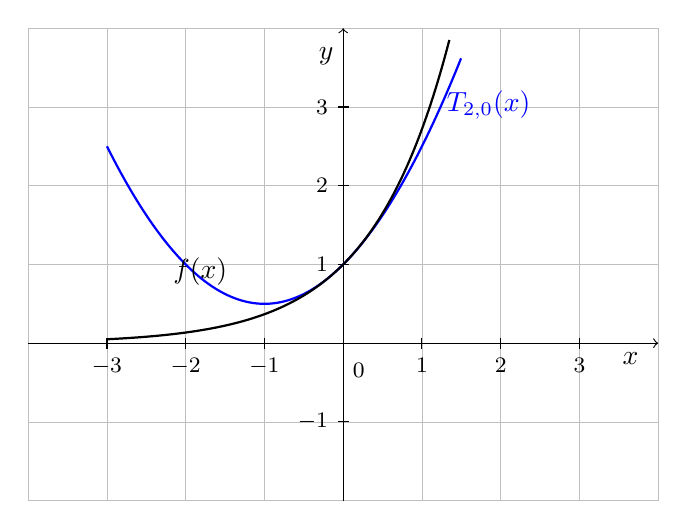
\begin{tikzpicture}

% Gitternetzlinien
\draw[xstep=1cm, ystep=1cm, very thin, color=lightgray] (-4,4) grid (4,-2);
% x-Achse
\draw[->] (-4,0) -- (4,0) node[below,xshift=-1em] {$x$}; 
%Zahlen auf x-Achse
\foreach \x in {-3,...,-1}
\draw[shift={(\x,0)},color=black] (0pt,2pt) -- (0pt,-2pt) node[below] {\footnotesize $\x$};
\foreach \x in {1,...,3}
\draw[shift={(\x,0)},color=black] (0pt,2pt) -- (0pt,-2pt) node[below] {\footnotesize $\x$};
% y-Achse 
\draw[->] (0,-2) -- (0,4) node[left,yshift=-1em] {$y$};%node[above left]
%Zahlen auf y-Achse
\foreach \y in {-1,...,-1}
\draw[shift={(0,\y)},color=black] (2pt,0pt) -- (-2pt,0pt) node[left] {\footnotesize $\y$};
\foreach \y in {1,...,3}
\draw[shift={(0,\y)},color=black] (2pt,0pt) -- (-2pt,0pt) node[left] {\footnotesize $\y$};
%Ursprung
\draw[color=black] (0pt,-10pt) node[right] {\footnotesize $0$};

\draw[thick,color=blue] plot[samples=200, domain=-3:1.5] 
(\x,{\x +1+0.5*\x*\x}) node[below, xshift=1em,yshift=-0.8em] {$T_{2,0}(x)$};

\draw[thick,color=black] plot[samples=200, domain=-3:1.35] 
(\x,{exp(\x)}) node[below, xshift=-9em,yshift=-7.5em]{$f(x)$};



\end{tikzpicture}\\
Die Annäherung um den Punkt $ x_0 $ ist bei $ n=2 $ besser als bei $ n=1 $.\\
\end{center}
\href{https://youtu.be/rOYhaQnvv98}{Video 08}\\
\underline{Für $ n=3 $ gilt:}\\
\begin{align*}
T_{3,0}&=\underbrace {1+x+\frac{1}{2}x^2}_{T_{2,0}}+\frac{f^{3}(0)}{3!}(x-0)^3\\
&=1+x+\frac{1}{2}x^2+\frac{1}{6}x^3\\
\end{align*}
\begin{center}
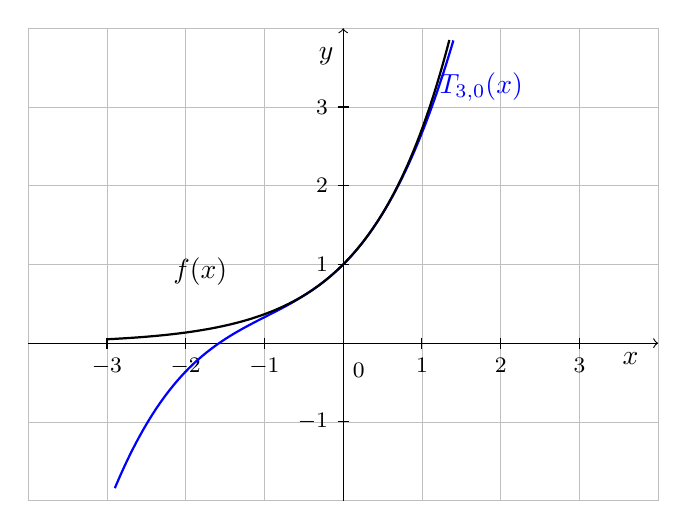
\begin{tikzpicture}

% Gitternetzlinien
\draw[xstep=1cm, ystep=1cm, very thin, color=lightgray] (-4,4) grid (4,-2);
% x-Achse
\draw[->] (-4,0) -- (4,0) node[below,xshift=-1em] {$x$}; 
%Zahlen auf x-Achse
\foreach \x in {-3,...,-1}
\draw[shift={(\x,0)},color=black] (0pt,2pt) -- (0pt,-2pt) node[below] {\footnotesize $\x$};
\foreach \x in {1,...,3}
\draw[shift={(\x,0)},color=black] (0pt,2pt) -- (0pt,-2pt) node[below] {\footnotesize $\x$};
% y-Achse 
\draw[->] (0,-2) -- (0,4) node[left,yshift=-1em] {$y$};%node[above left]
%Zahlen auf y-Achse
\foreach \y in {-1,...,-1}
\draw[shift={(0,\y)},color=black] (2pt,0pt) -- (-2pt,0pt) node[left] {\footnotesize $\y$};
\foreach \y in {1,...,3}
\draw[shift={(0,\y)},color=black] (2pt,0pt) -- (-2pt,0pt) node[left] {\footnotesize $\y$};
%Ursprung
\draw[color=black] (0pt,-10pt) node[right] {\footnotesize $0$};

\draw[thick,color=blue] plot[samples=200, domain=-2.9:1.4] 
(\x,{\x +1+0.5*\x*\x+0.17*\x*\x*\x}) node[below, xshift=1em,yshift=-0.8em] {$T_{3,0}(x)$};

\draw[thick,color=black] plot[samples=200, domain=-3:1.35] 
(\x,{exp(\x)}) node[below, xshift=-9em,yshift=-7.5em]{$f(x)$};



\end{tikzpicture}\\
Hier ist die Approximation in der Umgebung von $ x_0=0 $ noch besser.
\end{center}
Graphischer Vergleich der Taylorpolynome.\\
\begin{center}
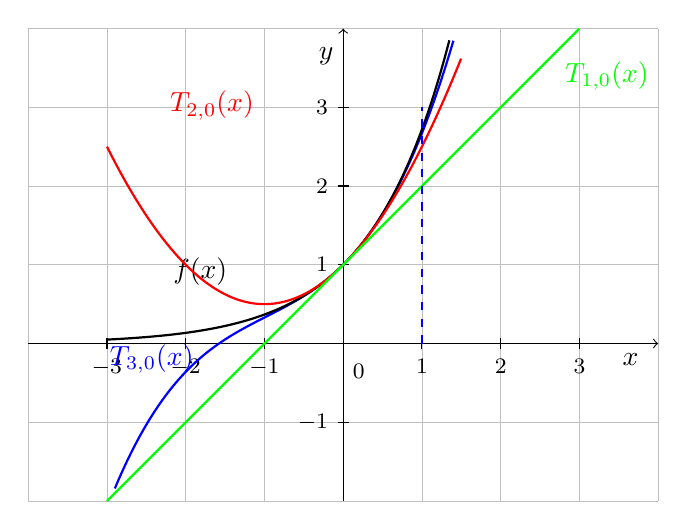
\begin{tikzpicture}

% Gitternetzlinien
\draw[xstep=1cm, ystep=1cm, very thin, color=lightgray] (-4,4) grid (4,-2);
% x-Achse
\draw[->] (-4,0) -- (4,0) node[below,xshift=-1em] {$x$}; 
%Zahlen auf x-Achse
\foreach \x in {-3,...,-1}
\draw[shift={(\x,0)},color=black] (0pt,2pt) -- (0pt,-2pt) node[below] {\footnotesize $\x$};
\foreach \x in {1,...,3}
\draw[shift={(\x,0)},color=black] (0pt,2pt) -- (0pt,-2pt) node[below] {\footnotesize $\x$};
% y-Achse 
\draw[->] (0,-2) -- (0,4) node[left,yshift=-1em] {$y$};%node[above left]
%Zahlen auf y-Achse
\foreach \y in {-1,...,-1}
\draw[shift={(0,\y)},color=black] (2pt,0pt) -- (-2pt,0pt) node[left] {\footnotesize $\y$};
\foreach \y in {1,...,3}
\draw[shift={(0,\y)},color=black] (2pt,0pt) -- (-2pt,0pt) node[left] {\footnotesize $\y$};
%Ursprung
\draw[color=black] (0pt,-10pt) node[right] {\footnotesize $0$};

\draw[thick,color=blue] plot[samples=200, domain=-2.9:1.4] 
(\x,{\x +1+0.5*\x*\x+0.17*\x*\x*\x}) node[below, xshift=-10.9em,yshift=-10.6em] {$T_{3,0}(x)$};

\draw[thick,color=black] plot[samples=200, domain=-3:1.35] 
(\x,{exp(\x)}) node[below, xshift=-9em,yshift=-7.5em]{$f(x)$};

\draw[thick,color=red] plot[samples=200, domain=-3:1.5] 
(\x,{\x +1+0.5*\x*\x}) node[below, xshift=-9em,yshift=-.8em] {$T_{2,0}(x)$};
\draw[thick,color=green] plot[samples=200, domain=-3:3] 
(\x,{\x +1}) node[below, xshift=1em,yshift=-0.8em] {$T_{1,0}(x)$};
\draw[thick,color=blue,dashed] (1,0)--(1,3) ;
\end{tikzpicture}\\
\end{center}
Bei $ x=1 $ kann man sehr gut die unterschiedlichen Fehler der Approximation ablesen.\\
Fehlerberechnung:\\
\begin{align*}
|T_{1,0}-f(1)|=|1+1-2,718|=0.718\\
|T_{2,0}-f(1)|=|1+1+\frac{1}{2}\cdot 1^2-2,718|=0.281\\
|T_{3,0}-f(1)|=|1+1+\frac{1}{2}\cdot 1^2+\frac{1}{6}\cdot 1^3-2,718|=0.051\\
\end{align*}
Den Fehler bei dem Taylorpolynom  $ T_{3,0} $ kann man graphisch bei $ x=1 $ schon nicht mehr ablesen.\\
\newpage
\noindent
\subsubsection{Die Taylorapproximation}
\href{https://youtu.be/sZeivAKBMa0}{Video 09}\\
Sei $ f: \mathbb{I}\longmapsto \mathbb{R} $ n-mal diffbar auf dem Intevall $  \mathbb{I} $ und sei $ x_0\in  \mathbb{I} $ dann gilt:\\
\begin{align*}
f(x)\approx T_{n.x_0}(x)\\
\end{align*}
Dieses Polynom entspricht genau der  Funktion $ f(x) $, wenn man den Fehler $ R_{n}(x) $ dem Polynom dazu addiert. Dann gilt:\\
\begin{align*}
f(x)=T_{n,x_0}(x)+R_{n}(x)=\sum\limits_{k=0}^{n}\frac{f^{k}(x_0)}{k!}(x-x_0)^k+R_n(x)\\
\end{align*}
Die Tayloapproximation entspricht: Polynom + Fehler.\\
Für diesen Fehler gilt:\\
\begin{align*}
\lim\limits_ {x\to x_0}\frac{R_n(x)}{(x-x_0)^n}=0\\
\end{align*}
Dies bedeutet, obwohl $ \frac{1}{(x-x_0)^n} $ schon sehr schnell gegen Null geht (wegen den hoch n), dass der Zähler (Fehler)  noch schneller gegen Null läuft.\vspace*{4mm}\\
Ist $ f^{n+1} $ n-mal diffbar, dann gilt, wenn $ a $ zwischen $ x $ und $ x_0 $ liegt :\\
\begin{center}
Restglied von Lagrange\\
$\boxed{R_n(x)=\frac{f^{n+1}(a)}{(n+1)!}(x-x_0)^{n+1}\;\;a\in[x,x_0]}$
\end{center}
\subsubsection{Beispiel zur Taylorapproximation}
\href{https://youtu.be/T6jBJ9BVPg8}{Video 10}\\
Bestimme die Taylorapproximation $ T_{1,x_0} $ von  $ f(x)=\mathrm{e}^x $ mit $ x_0=0 $.\\
Es gilt:\\
\begin{align*}
f(x)=\mathrm{e}^x&=T_{1,x_0}+R_1(x)\\
&=f(0)+\frac{f'(0)}{1!}(x-0)^1+R_1(x)\\
&=1+x+R_1(x)\\
\end{align*}
Restglied $ R_{1}(x) $ bestimmen:\\
Es gilt:\\
\begin{align*}
R_n(x)=\frac{f^{n+1}(a)}{(n+1)!}(x-x_0)^{n+1}\\
\end{align*}
\begin{align*}
R_1(x)=\frac{f''(a)}{2!}(x-x_0)^2=\frac{\mathrm{e}^a}{2}x^2\\
\end{align*}
\textbullet\;\;Es muß gelten:\\
\begin{align*}
\lim\limits_ {x\to x_0}\frac{R_1(x)}{(x-x_0)^1}=0
\end{align*}
\begin{align*}
\lim\limits_ {x\to 0}=\frac{\frac{\mathrm{e}^a}{2}x^2}{x}=\lim\limits_ {x\to 0}\frac{\mathrm{e}^a}{2}x=0
\end{align*}
\textbullet\;\;Restglied abschätzen:\\
\begin{quote}
1. Für $ x\in \;[0,2] $:\\
\begin{align*}
R_1(x)=\frac{\mathrm{e}^a}{2}x^2\leq \frac{\mathrm{e}^a}{2}\cdot 2=\mathrm{e}^a\cdot 2\\
\end{align*}
Da $ a $ zwischen $ x_0 $ und $  x $ liegt, gilt:\\
Abschätzung nach oben:\\
\begin{align*}
R_1(x)=\frac{\mathrm{e}^a}{2}x^2\leq \mathrm{e}^a\cdot 2 < \mathrm{e}^2\cdot 2
\end{align*}
Abschätzung nach unten:\\
\begin{align*}
0=\mathrm{e}^0\cdot 0<R_1(x)&=\frac{\mathrm{e}^a}{2}x^2\leq \mathrm{e}^a\cdot 2 < \mathrm{e}^2\cdot 2\\
0<R_1(x)& < \mathrm{e}^2\cdot 2\\
\end{align*}
2. Für $ x\in \;[0,200] $:\\
\begin{align*}
R_1(x)=\frac{\mathrm{e}^a}{2}x^2\leq \frac{\mathrm{e}^a}{2}\cdot 200^2<\frac{\mathrm{e}^{200}}{2}\cdot 200^2
\end{align*}
Hier ist der Fehler riesengroß!\\

\end{quote}

\subsubsection{Aufgabe 1 zur Taylorapproximation Teil I u. Teil II}
\href{https://youtu.be/NbAlqm36CTo}{Video 11}\\
Berechne das Taylorpolynom 3. Grades von $ f(x)=\cos(x) $ in $ x_0=\pi $ und approximiere $ f(3)=\cos(3) $ damit. Schätze danach den Fehler ab.\\
\textbullet\;\; Bestimmung der Ableitung $ f'(x),\;f''(x),\;f^{(3)}(x) $.\\
\begin{align*}
f(x)&=\cos(x)\\
f'(x)&=-\sin(x)\\
f''(x)&=-\cos(x)\\
f^{(3)}(x)&=\sin(x)\\
\end{align*}
\textbullet\;\; Bestimmung von $ f(\pi),\; f'(\pi),\; f''(\pi),\; f^{(3)}(\pi) $.\\
\begin{align*}
f(\pi)&=-1\\
f'(\pi)&=0\\
f''(\pi)&=1\\
f^{(3)}(\pi)&=0
\end{align*}
\textbullet\;\; Einsetzen in das Taylorpolynom.\\
\begin{quote}
\begin{align*}
T_{3,\pi}&=\sum\limits_{k=0}^{3}\frac{f^k(\pi)}{k!}(x-\pi)^k=\frac{f(\pi)}{0!}(x-\pi)^0+\frac{f'(\pi)}{1!}(x-\pi)^1+\frac{f''(\pi)}{2!}(x-\pi)^2+\frac{f^{(3)}(\pi)}{3!}(x-\pi)^3\\
&=-1+\frac{1}{2}(x-\pi)^2\\
\end{align*}
\end{quote}
\textbullet\;\;Für $ \cos(3) $ approximiert gilt dann:\\
\begin{align*}
&T_{3,\pi}\approx-1+\frac{1}{2}(3-\pi)^2=-0.9899757\\ 
&\text{mit Taschenrechner }\;\;\cos(3)=0.9899924\\
\end{align*}
\href{https://youtu.be/sWuEka8oIQY}{Video 12}\\
\textbullet\;\;Fehlerabschätzung:\\
\begin{quote}
Es gilt:\\
\begin{align*}
&f(x)=T_{3,\pi}(x)+R_3(x)\\
&\Leftrightarrow\\
&R_3(x)=f(x)-T_{3,\pi}(x)\\
\end{align*}
Mit dem Restglied von Lagrange wird der Fehler abgeschätzt.\\
\begin{align*}
R_3(x)=\frac{f^{(4)}(a)}{4!}(x-x_0)^{4}\;\;a\in[x,x_0]\\
\end{align*}
\begin{align*}
f^{(4)}&=\cos(x)\\
x&=3\\
x_0&=\pi\\
\end{align*}
Bestimmung von $ a $:\\
\begin{align*}
&a\in[3,\pi]\\
&\cos(3)=-0.989\\
&\cos(\pi)=-1
\end{align*}
Da der Fehler absolut ist, wählt man den $ \cos(a) $ so, dass er den größten Fehler hat.\\
Dies gilt bei $ \cos(a)=\cos(\pi)=-1 $ also $ a=\pi $.\\
Dann gilt:\\
\begin{align*}
\big|R_{3}(x)\big|<\bigg|\frac{\cos(a)}{4!}(3-\pi)^4\bigg|<\bigg|\frac{\cos(\pi)}{4!}(3-\pi)^4\bigg|=\bigg|\frac{-(3-\pi)^4}{4!}\bigg|
\end{align*}
Dieser Fehler ist hier schon sehr klein!\\
\end{quote}
\subsubsection{Aufgabe 1 zur Taylorapproximation Teil I u. Teil II}
\href{https://youtu.be/iHpIwbXhDLs}{Video 13}\\
Bestimme für $ f(x)=\sqrt{2+x} $ das Taylorpolynom 3.Grades in $ x_0=-1 $.\\
Schätze den Fehler für $ x\in\;]-\frac{1}{4},\frac{1}{4}[ $ ab.\\
\textbullet\;\; Bestimmung der Ableitung $ f'(x),\;f''(x),\;f^{(3)}(x) $.\\
\begin{align*}
f(x)&=\sqrt{2+x}\\
f'(x)&=\frac{1}{2\sqrt{2+x}}\\
f''(x)&=\bigg(\frac{1}{2}(2+x)^{-\frac{1}{2}}\bigg)'=-\frac{1}{4}(2+x)^{-\frac{3}{2}}=-\frac{1}{4}\frac{1}{\sqrt{(2+x)^3}}\\
f^{(3)}(x)&=\bigg(-\frac{1}{4}(2+x)^{-\frac{3}{2}}\bigg)'=\frac{3}{8}(2+x)^{-\frac{5}{2}}=\frac{3}{8}\frac{1}{\sqrt{(x+2)^{5}}}\\
\end{align*}
\textbullet\;\; Bestimmung von $ f(-1),\; f'(-1),\; f''(-1),\; f^{(3)}(-1) $.\\
\begin{align*}
f(-1)&=1\\
f'(-1)&=\frac{1}{2}\\
f''(-1)&=-\frac{1}{4}\\
f^{3}(-1)&=\frac{3}{8}\\
\end{align*}
\textbullet\;\; Einsetzen in das Taylorpolynom.\\
\begin{align*}
T_{3,-1}&\approx \frac{f(-1)}{0!}+\frac{f'(-1)}{1!}(x+1)+\frac{f''(-1)}{2!}(x+1)^2+\frac{f^{3}(-1)}{3!}(x+1)^3\\
&\approx 1+\frac{1}{2}(x+1)-\frac{1}{8}(x+1)^2+\frac{1}{16}(x+1)^3\\
\end{align*}
\href{https://youtu.be/KGQM0psy20I}{Video 14}\\
\textbullet\;\;Mit dem Restglied von Lagrange wird der Fehler abgeschätzt.\\
\begin{align*}
\big|R_3(x)\big|=\bigg|\frac{f^{(4)}(a)}{4!}(x-x_0)^{4}\bigg|\;\;a\in[x,x_0], \; x\in\;]-\genfrac{}{}{}{2}{1 }{4 },\genfrac{}{}{}{2}{1 }{4 }[\\
\end{align*}
\begin{align*}
f^{(4)}(a)=\bigg(\frac{3}{8}\frac{1}{\sqrt{(x+2)^{5}}}\bigg)'=-\frac{15}{16}\frac{1}{\sqrt{(2+a)^7}}
\end{align*}
\begin{align*}
\big|R_3(x)\big|=\bigg|-\frac{15}{16}\frac{1}{\sqrt{(2+a)^7}4!}(x+1)^4\bigg|
\end{align*}
\begin{quote}
Abschätzen des Terms $a\in [-1,x]$ und $ x\in\;]-\frac{1}{4},\frac{1}{4}[ $\\
Für $ x=\frac{1}{4} $ wird der Term $ (x+1)^4 $ am größten.\\
Für $ a=-1 $ wird der Nenner $ \sqrt{(2+a)^7} $ am kleinsten und der Bruch am größten.\\
Der größtmögliche Fehler ist dann:\\
\begin{align*}
\big|R_3(x)\big|<\bigg|-\frac{15}{16}\frac{1}{\sqrt{(2-1)^7}4!}\bigg(\frac{1}{4}+1\bigg)^4\bigg|=\frac{5\cdot3}{4\cdot4}\cdot\frac{1}{4\cdot3\cdot 2}\cdot\frac{5^4}{4^4}=\frac{5^5}{2\cdot4^7}\\
\end{align*}


\end{quote}
\subsection{Das hinreichende Kriterium für Extrema}
\href{https://youtu.be/qZN36TCHIVw}{Video 15}\\
Sei $ f:  \mathbb{I}\longmapsto \mathbb{R} $ auf dem Intervall $  \mathbb{I} $ n- mal differenzierbar.\\
Sei $ x_0\in  \mathbb{I} $ ein innerer Punkt.\\
Ist $ f'(x_0)=f''(x_0) =\ldots =f^{n-1}(x_0)=0$ und $ f^{n}(x_0)\neq 0 $ dann gilt:\\
\begin{quote}
(i)\;\; Ist $ n $ ungerade $ \Rightarrow  f$ kein Extrema in $ x_0 $\\
(ii)\;\;Ist $ n $ gerade dann gilt für:
\begin{quote}
1. $f^n > 0 \Rightarrow f$ lokales Minimum in $ x_0 $\\
2. $f^n < 0 \Rightarrow f$ lokales Maximum in $ x_0 $\\
\end{quote}
\end{quote}
Beispiel:\\
\textbullet \;\;$ f:\mathbb{R}\longmapsto[0,\infty[\;\;\text{mit }\;\; f(x)=x^2 $\\
\begin{quote}
$ f $ hat in $ x_0=0 $ ein lokales Minimum, denn:\\
\begin{align*}
f'(x_0)&=2x_0=0\\
f''(x_0)&=2>0\\
\end{align*}
\end{quote}
\newpage
\noindent
\textbullet\;\;$\overset{\AC}{f}: \mathbb{R}\longmapsto\mathbb{R}\;\;\text{mit }\;\;\overset{\AC}{f}(x)=x^3$\\
\begin{quote}
$\overset{\AC}{f}$ hat in $ x_0=0 $ kein Extrema, denn:\\
\begin{align*}
\overset{\AC}{f'}(x_0)&=3x_0^2=0=6x_0=\overset{\AC}{f''}(x_0)\\
\overset{\AC}{f^{3}}(x_0)&=6\\
\end{align*}
Da $ \overset{\AC}{f^{3}}(x_0)=6\neq 0 $ ungerade ist hat $\overset{\AC}{f}  $ in $ x_o $ kein Extrema.\\
\end{quote}
\subsubsection{Aufgabe 1 zum hinreichenden Kriterium für Extrema Teil I u. Teil II}
\href{https://youtu.be/Anjy9d6Qu2Y}{Video 16}\\
Bestimme alle lokalen und globalen Extrema von $ f:\;]-\frac{1}{2},3]\;\longmapsto \mathbb{R} $ mit $ f(x)=\mathrm{e}^{2x^3+3x^2} $.\\
\\
(I) Untersuchung der inneren Punkte: $ x\in\;]-\frac{1}{2},3] $\\
\begin{quote}
1. Bestimmung von $ f'(x) $ und die Nullstellen von $ f'(x) $.\\
\begin{quote}
\begin{align*}
f'(x)=\mathrm{e}^{2x^3+3x^2}(6x^2+6x)=0\\
\end{align*}
$ \mathrm{e}^{2x^3+3x^2} $ ist immer positiv.\\
$ f'(x)=0 $, wenn$ (6x^2+6x)=0 $\\
\begin{align*}
&6x^2+6x=0\\
&\Leftrightarrow\\
&\Leftrightarrow 6(x^2+x)=0\\
&\Leftrightarrow 6x(x+1)=0\\
&x_1=0\\
&x_2=-1\\
\end{align*}
$ x_2 \notin \;]-\genfrac{}{}{}{2}{1 }{2 },3] $\\
Die einzige potentielle Extremstelle im Intervall $ ]-\frac{1}{2},3] $ ist $x_1=0  $\\
\end{quote}
2. $ x_1=0 $ in 2. Ableitung einsetzen.\\
\begin{quote}
\begin{align*}
f''(x)&=\mathrm{e}^{2x^3+3x^2}(6x^2+6x)^2+\mathrm{e}^{2x^3+3x^2}(12x+6)\\
f''(x_1)&=f''(0)=0+\mathrm{e}^0\cdot 6=6>0
\end{align*}
Also hat $ f $ in $ x_1 $ ein lokales Minimum.\\
\end{quote}
\end{quote}
\href{https://youtu.be/xKTPSfSrtGo}{Video 17}\\
(II) Randwertbetrachtung und Grenzwertbetrachtung an den Rändern vom Intervall  $ x\in\;]-\frac{1}{2},3] $ .\\
\begin{quote}
1. An der Stelle $ x=3 $.
\begin{align*}
&f(x)=\mathrm{e}^{2x^3+3x^2}\\
&f(3)=\mathrm{e}^{2\cdot3^3+3\cdot3^2}=\mathrm{e}^{3\cdot27}\\
\end{align*}
2. Grenzwert an der Stelle $ x\mapsto -\frac{1}{2} $
\begin{align*}
\lim\limits_ {\substack{x \to -\frac{1}{2} \\ x>-\frac{1}{2}}}\mathrm{e}^{-2\cdot \frac{1}{8}+3\cdot\frac{1}{4}}=\mathrm{e}^{\frac{1}{2}}=\sqrt{e}\\
\end{align*}
\end{quote}
Fazit:\\
\begin{align*}
f(0)=\mathrm{e}^{2\cdot 0+3\cdot 0}=\mathrm{e}^0=1<\sqrt{e}<\mathrm{e}^{3\cdot 27}\\
\end{align*}
D.h.:\\
In $ x_1=0 $ hat $ f $ globales Minimum.\\
In $ x_2=3 $ hat $ f $ globales Maximum.
\subsubsection{Aufgabe 2 zum hinreichenden Kriterium für Extrema}
\href{https://youtu.be/JRMKUC_oVdM}{Video 18}\\
Bestimme alle lokalen und globalen Extrema von: $ \mathbb{R}\longmapsto \mathbb{R} $ mit 
$f(x) =     \left\{ \begin{array}{rcl}
\mathrm{e}^{6x^2} & \mbox{für} &  x\geq 0\\
6x^2+1 & \mbox{für} & x<0 \\

\end{array}\right.$\\
$ f(x) $ ist stetig und bis zur 2.Ableitung diffbar.\\
\\
Nullstellen der 1. Ableitung.\\
\begin{center}
$f'(x) =     \left\{ \begin{array}{rcl}
\mathrm{e}^{6x^2}\cdot12x & \mbox{für} & x\geq0\\
12x & \mbox{für} & x< 0 \\

\end{array}\right.$\\
\end{center}
\begin{align*}
f'(x)=0\Leftrightarrow \mathrm{e}^{6x^2}\cdot 12x\Rightarrow x_1=0\\
\end{align*}
Potenzielle Extremstelle ist $ x_1=0 $\\
$ x_1=0 $ in $ f''(x) $ einsetzen.\\
\begin{center}
$f''(x) =     \left\{ \begin{array}{rcl}
\mathrm{e}^{6x^2}(\cdot12x)^2+\mathrm{e}^{6x^2}\cdot12 & \mbox{für} & x\geq0\\
12 & \mbox{für} & x< 0 \\

\end{array}\right.$\\
\end{center}
\begin{align*}
&f''(0)=\mathrm{e}^{6\cdot 0^2}(\cdot12\cdot 0)^2+\mathrm{e}^{6\cdot 0^2}\cdot12=12>0\\
&\Rightarrow f\;\;\text{hat in  }\;\;x_1\;\;\text{ein lokales Minimum }\\
\end{align*}
Grenzwertbetrachtung:\\
\begin{align*}
&\text{\textbullet} \;\;\lim\limits_ {x\to\infty}f(x)=\lim\limits_ {x\to\infty}\mathrm{e}^{6x^2}=\infty\\
&\text{\textbullet }\;\;\lim\limits_ {x\to -\infty}f(x)=\lim\limits_ {x\to -\infty}6x^2+1=\infty\\
\end{align*}
Fazit: 
$ f $ hat in $ x_1 $ ein globales Minimum.
\\
\\
Bemerkung:
Bei der Grenzwert- oder Randwertbetrachten immer die $ \mathbb{D}_f $ und $ \mathbb{W}_f $ beachten, damit man richtig zwischen globalen und lokalen Maximun oder Minimum beurteilt.\\
Z.B:
\begin{align*}
\mathbb{R}&\longmapsto \mathbb{R}\\
[a,b]&\longmapsto ]a,b[\\
\mathbb{R}&\longmapsto ]a,b]\\
\end{align*}


